\chapter{GIS}
A rank of ranks study was done on 16 poverty and 16 development
features from AFDB/OCED 2007 data on 53 African Nations.  Taking
missing values into account - countries scores were calculated by
ranking across all features.  The resulting data set was imported
to ESRI ArcMap software to produce the poverty and development
heat maps.  The obvious spatial correlation is demonstrated in
Moran Scatterplots of the heat map data.

Ranking countries is a old and open problem.  See \footn{Munda G.,
Nardo M. (2005), "Non-compensatory composite indicators for
ranking countries: a defensible setting," EUR 21833 EN, European
Commission.} for a good background discussion.  Poverty and
development country ranks were calculated by ranking the
unweighted sum of the feature ranks \footn{Tools for Composite
Indicators Building. Nardo M., Saisana M., Saltelli A. and
Tarantola S. (2005) European Commission, EUR 21682 EN, Institute
for the Protection and Security of the Citizen, JRC Ispra,
Italy.}. The tables below list the
features used.\\\\

\begin{tabular}{|c c|}
  \hline
  % after \\: \hline or \cline{col1-col2} \cline{col3-col4} ...
  Development Features & \\
  \hline
GDP based on PPP valuation &     GDP per Capita   \\
  Annual real GDP Growth & FDI Inflow 2005 (\$ million) \\
Share of Consumption Lowest 10\%  &   Telcom Main Line (Per
100)2005 \\  com Mobile Lines (Per 100) 2005 & Water supply coverage Total  2004 \\
Water supply coverage Urban 2004 & Water supply coverage Rural
2004 \\ Sanitation coverage Total  2004 &   Sanitation coverage Urban 2004 \\
 Sanitation coverage Rural 2004 & Number of Products Accounting for $>$ 75\%
 Exports
 \\ GNI per capita, Atlas method (current US\$) &  2006 Softening of
 Regime \\
\hline
\end{tabular}
\\\\\\

\begin{tabular}{|c c|}
  \hline
  % after \\: \hline or \cline{col1-col2} \cline{col3-col4} ...
   Poverty Features & \\
  \hline
Population growth \% 2000-2005 & PopulationGrowth Rate 2005-2010\\
Infant Mortality /1000 & Mortality Under Age 5\\
Gini Coefficient & Share of Consumption Highest 10\% \\
Estimated adult illiteracy rate (\%) & AIDS Prevalence \\
Corruption Index (0-1) & Inflation 2005 \\
Inflation 2006(e) & Inflation 2007(p) \\
Inflation 2008(p) & 2005 Change in Political Troubles \\
2006 Change In Political Troubles & 2006 Hardening of Regime\\
\hline
\end{tabular}

The two heat maps below show the rankings of 53 African nations in
a larger data set.\footn{AfDB/OECD 2007 Statistical Annex} Note
missing values (dark blue) for many of the absolute poverty
measures these were left out of the rank study.  Missing values
were handled by exclusion instead of imputation.  Missing values
bias rank algorithms towards a higher false negative rate.
Spatially interpolating feature values from neighboring countries
works when the feature can be spatially modelled, say AIDS rate.

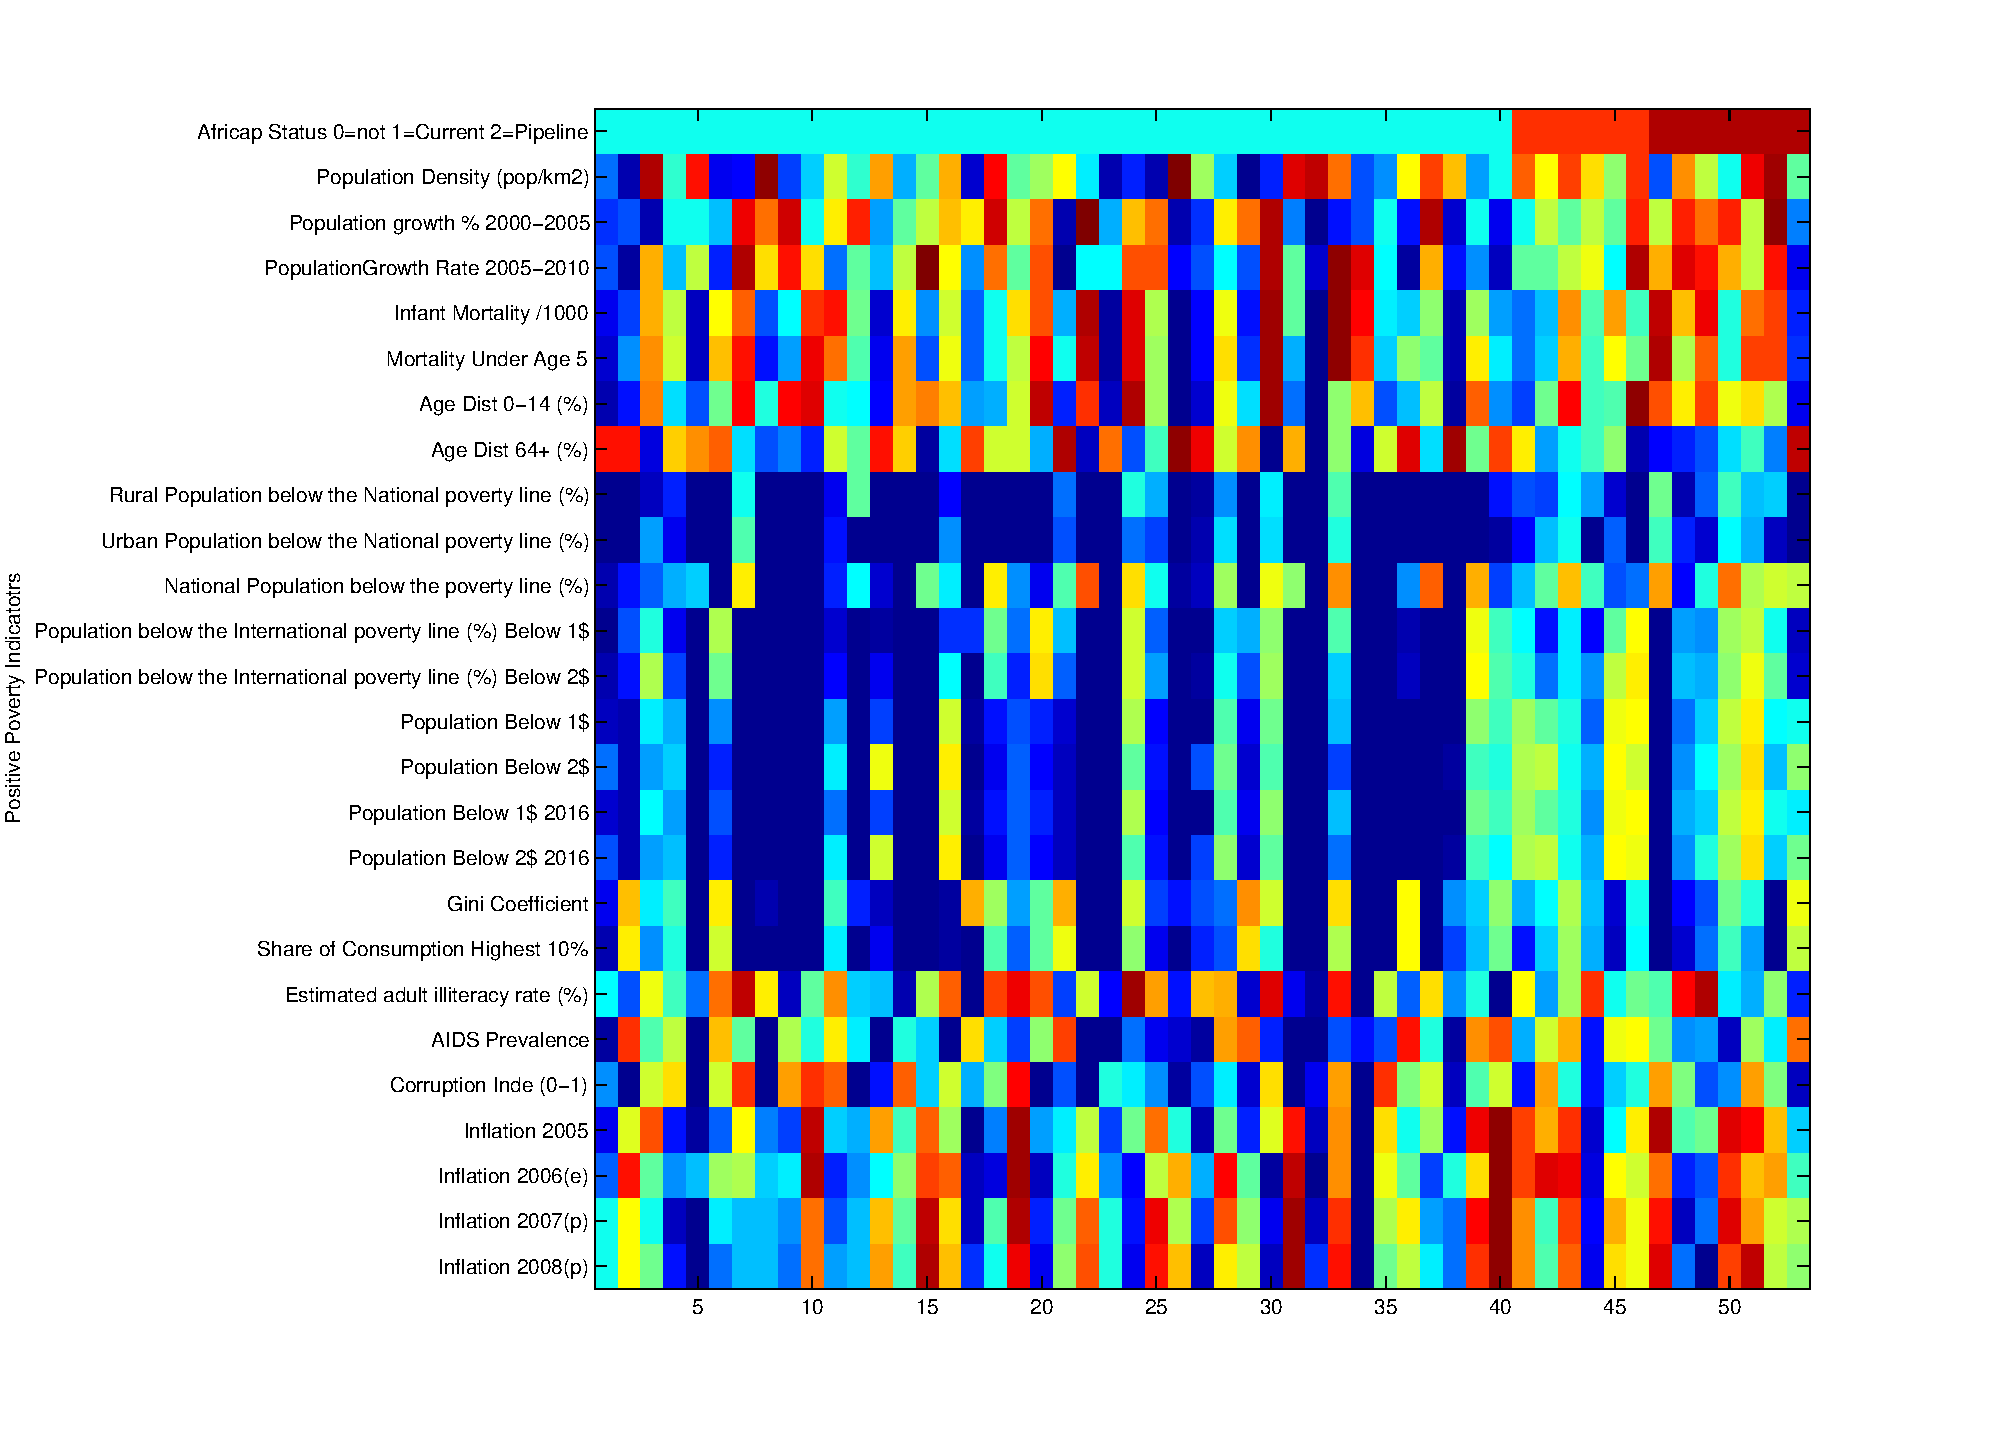
\includegraphics[width=5in]{Images/GIS/PositivePovertyIndicatorHeatMap.pdf}

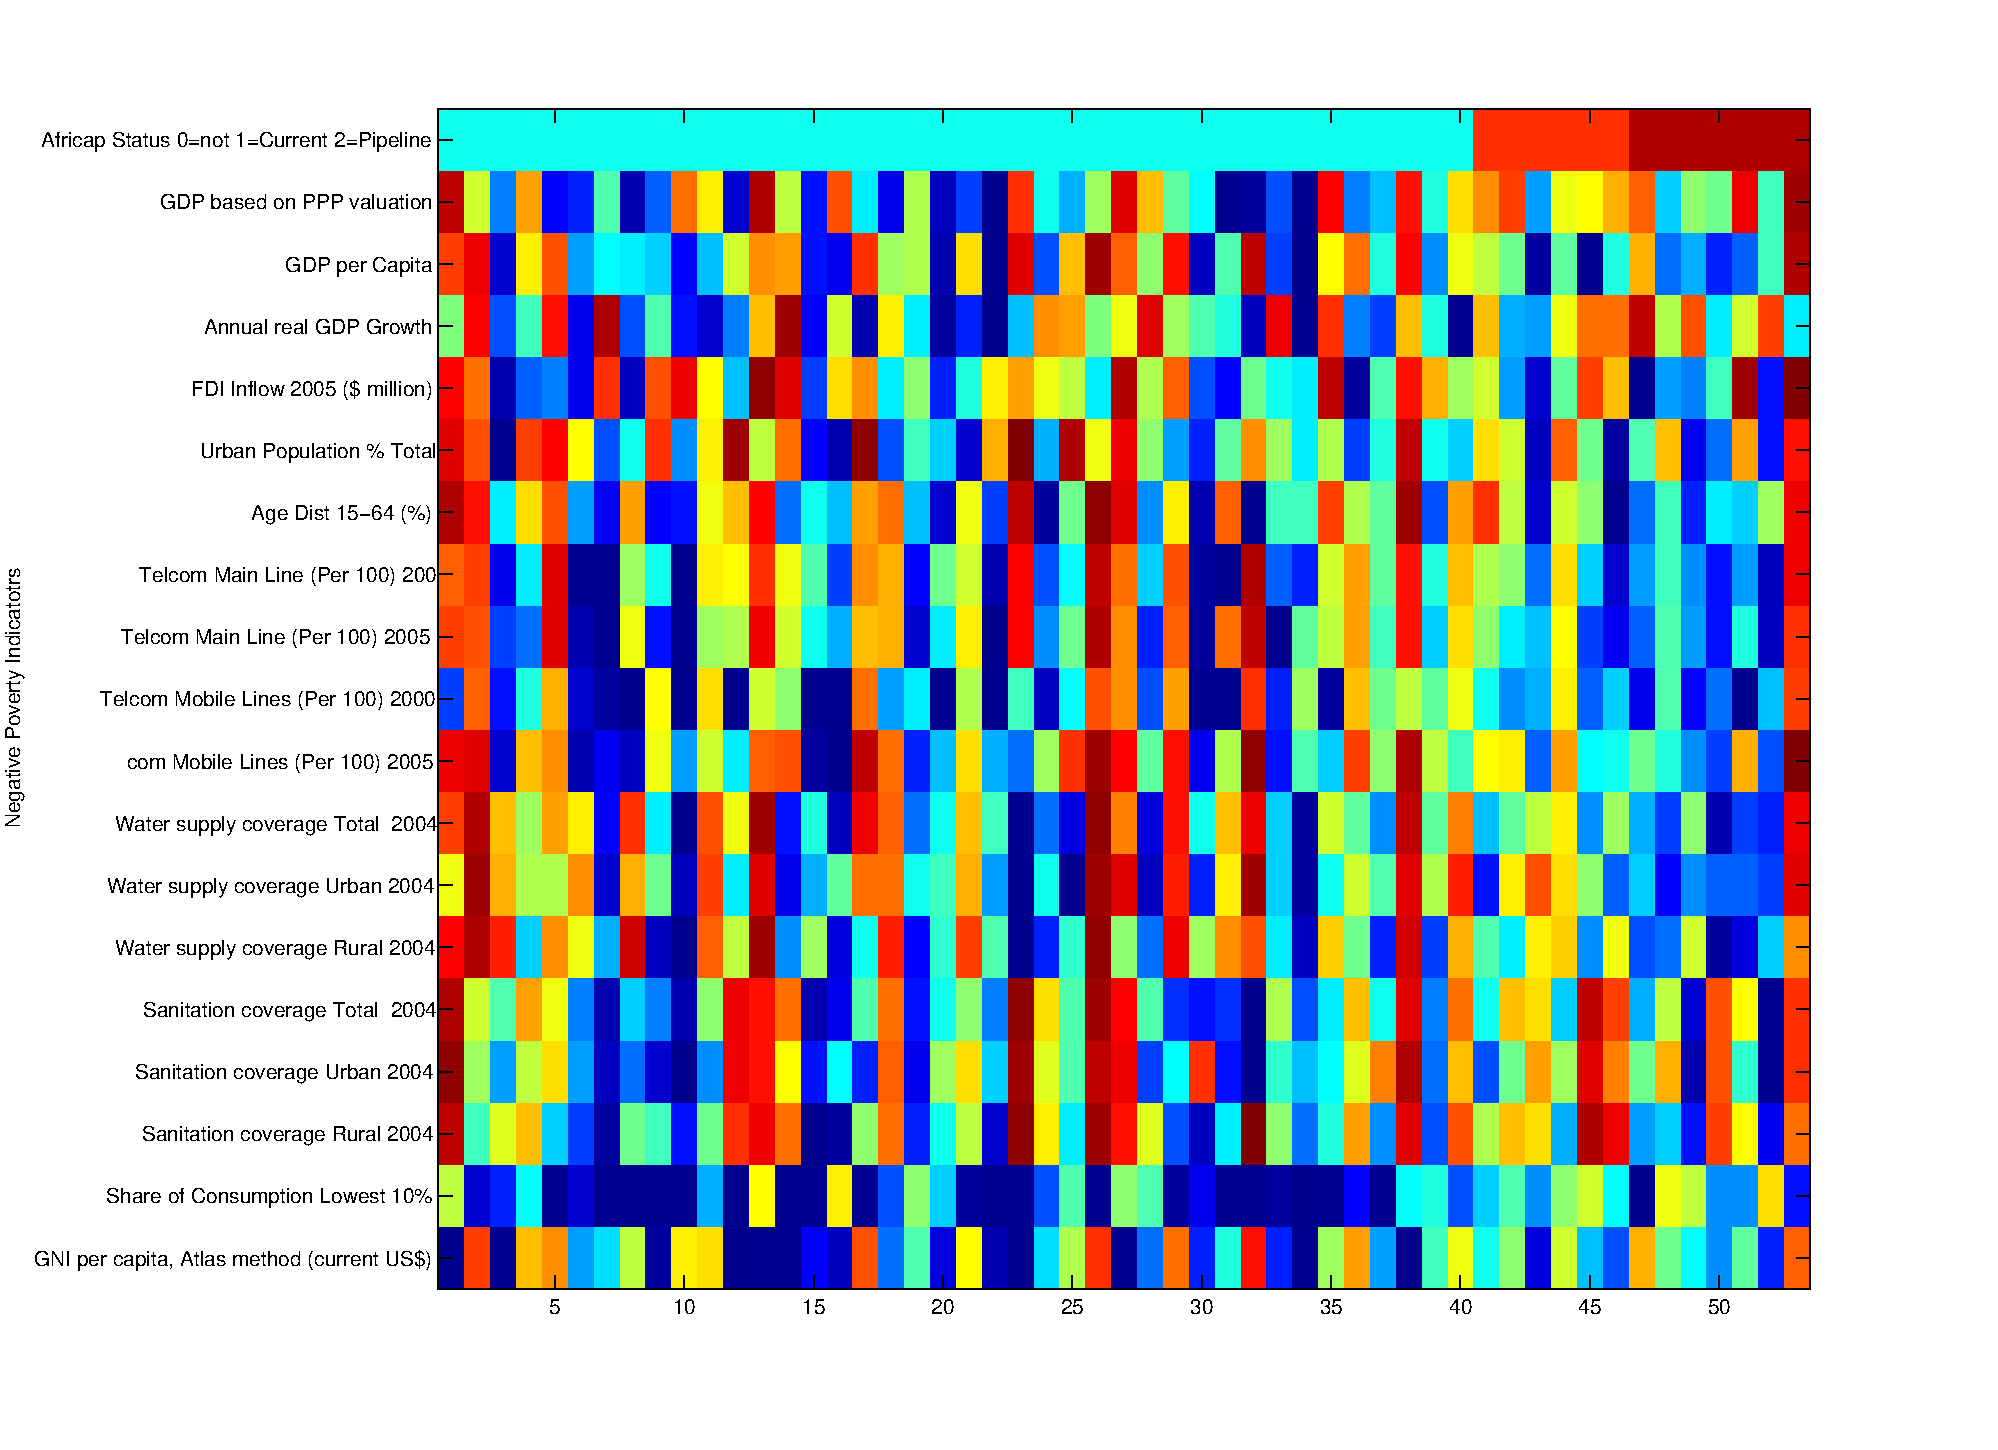
\includegraphics[width=5in]{Images/GIS/NegativePovertyIndicatorHeatMap.pdf}

\newpage


\newpage
African poverty heat map.

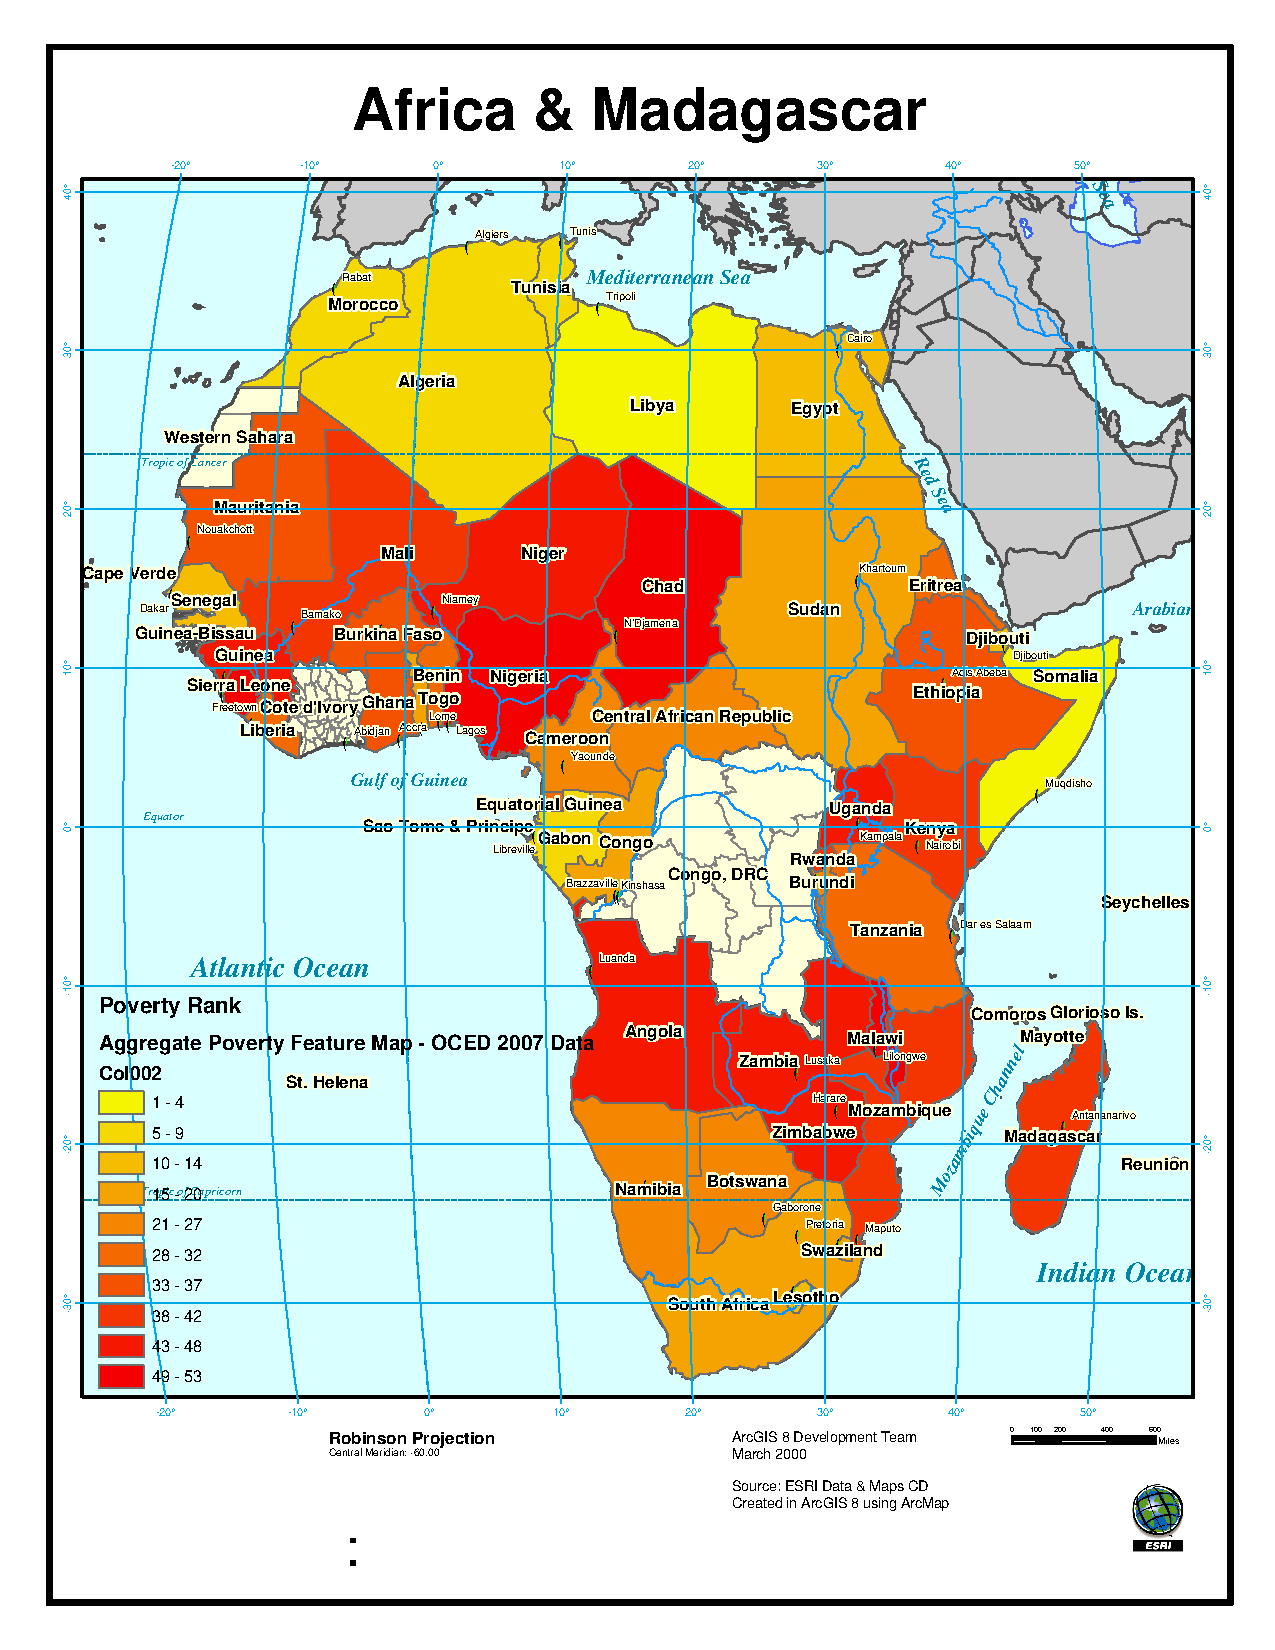
\includegraphics[width=6in]{Images/GIS/PovertyFeatureMapV0.pdf}

\newpage

African development heat map.

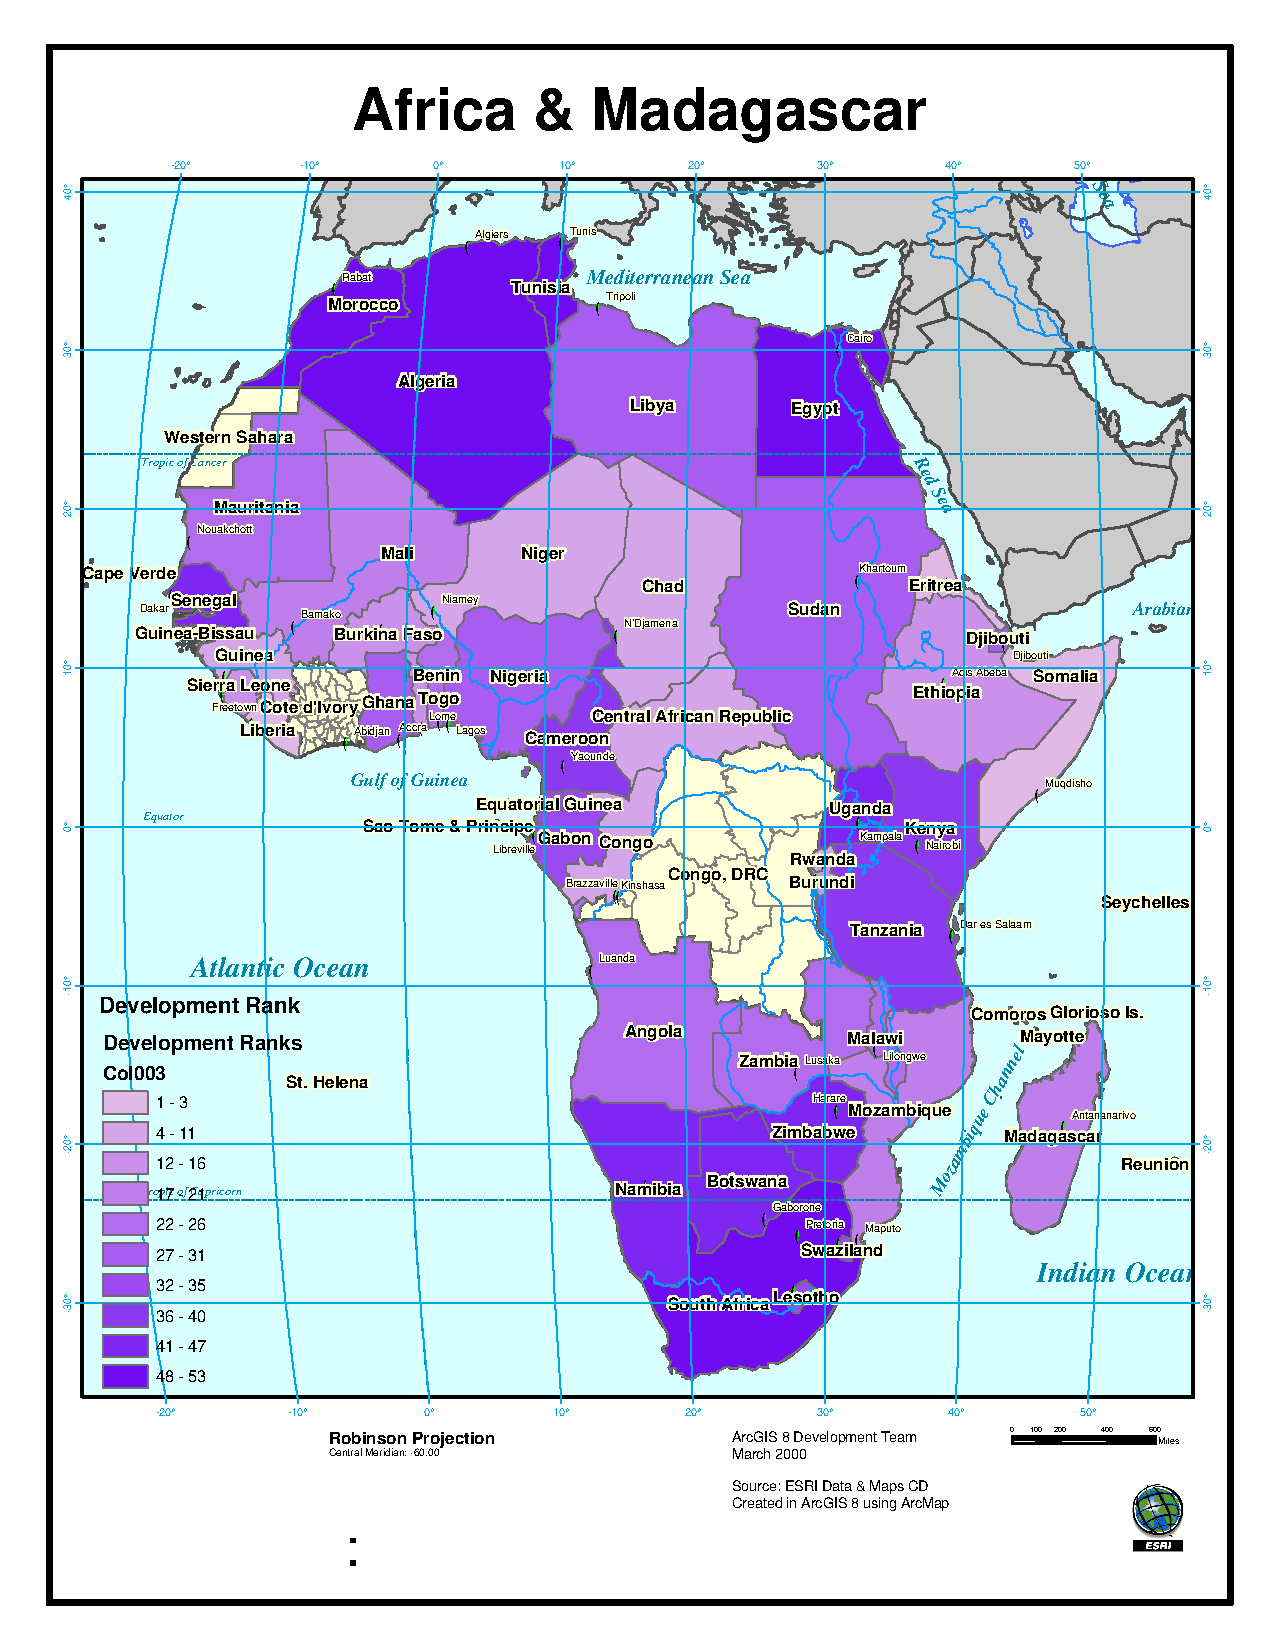
\includegraphics[width=6in]{Images/GIS/PovertyFeatureMapV1Development.pdf}
\newpage

Adding Habitat to the poverty heat map.

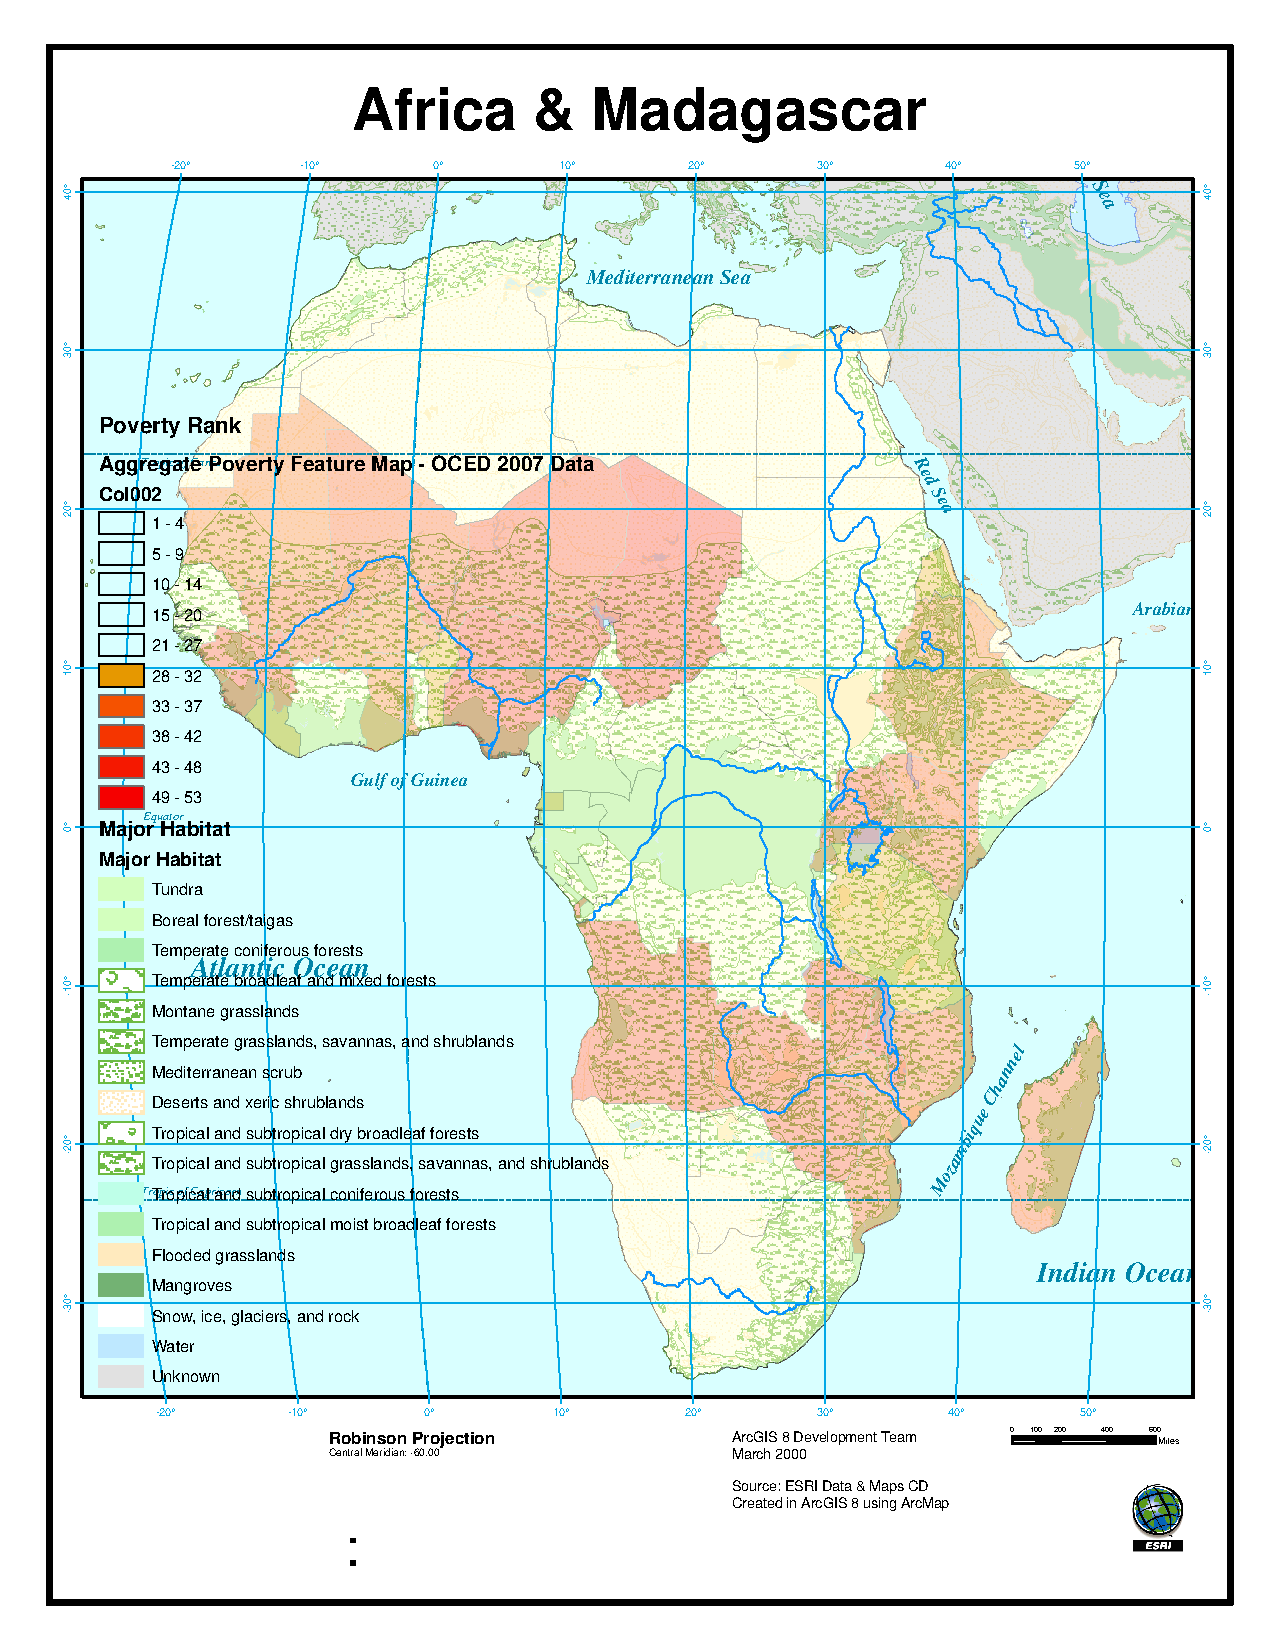
\includegraphics[width=6in]{Images/GIS/PovertyFeatureMapV3_Poverty_Habitat.pdf}

\newpage

Overlap of high poverty rank and low development rank.

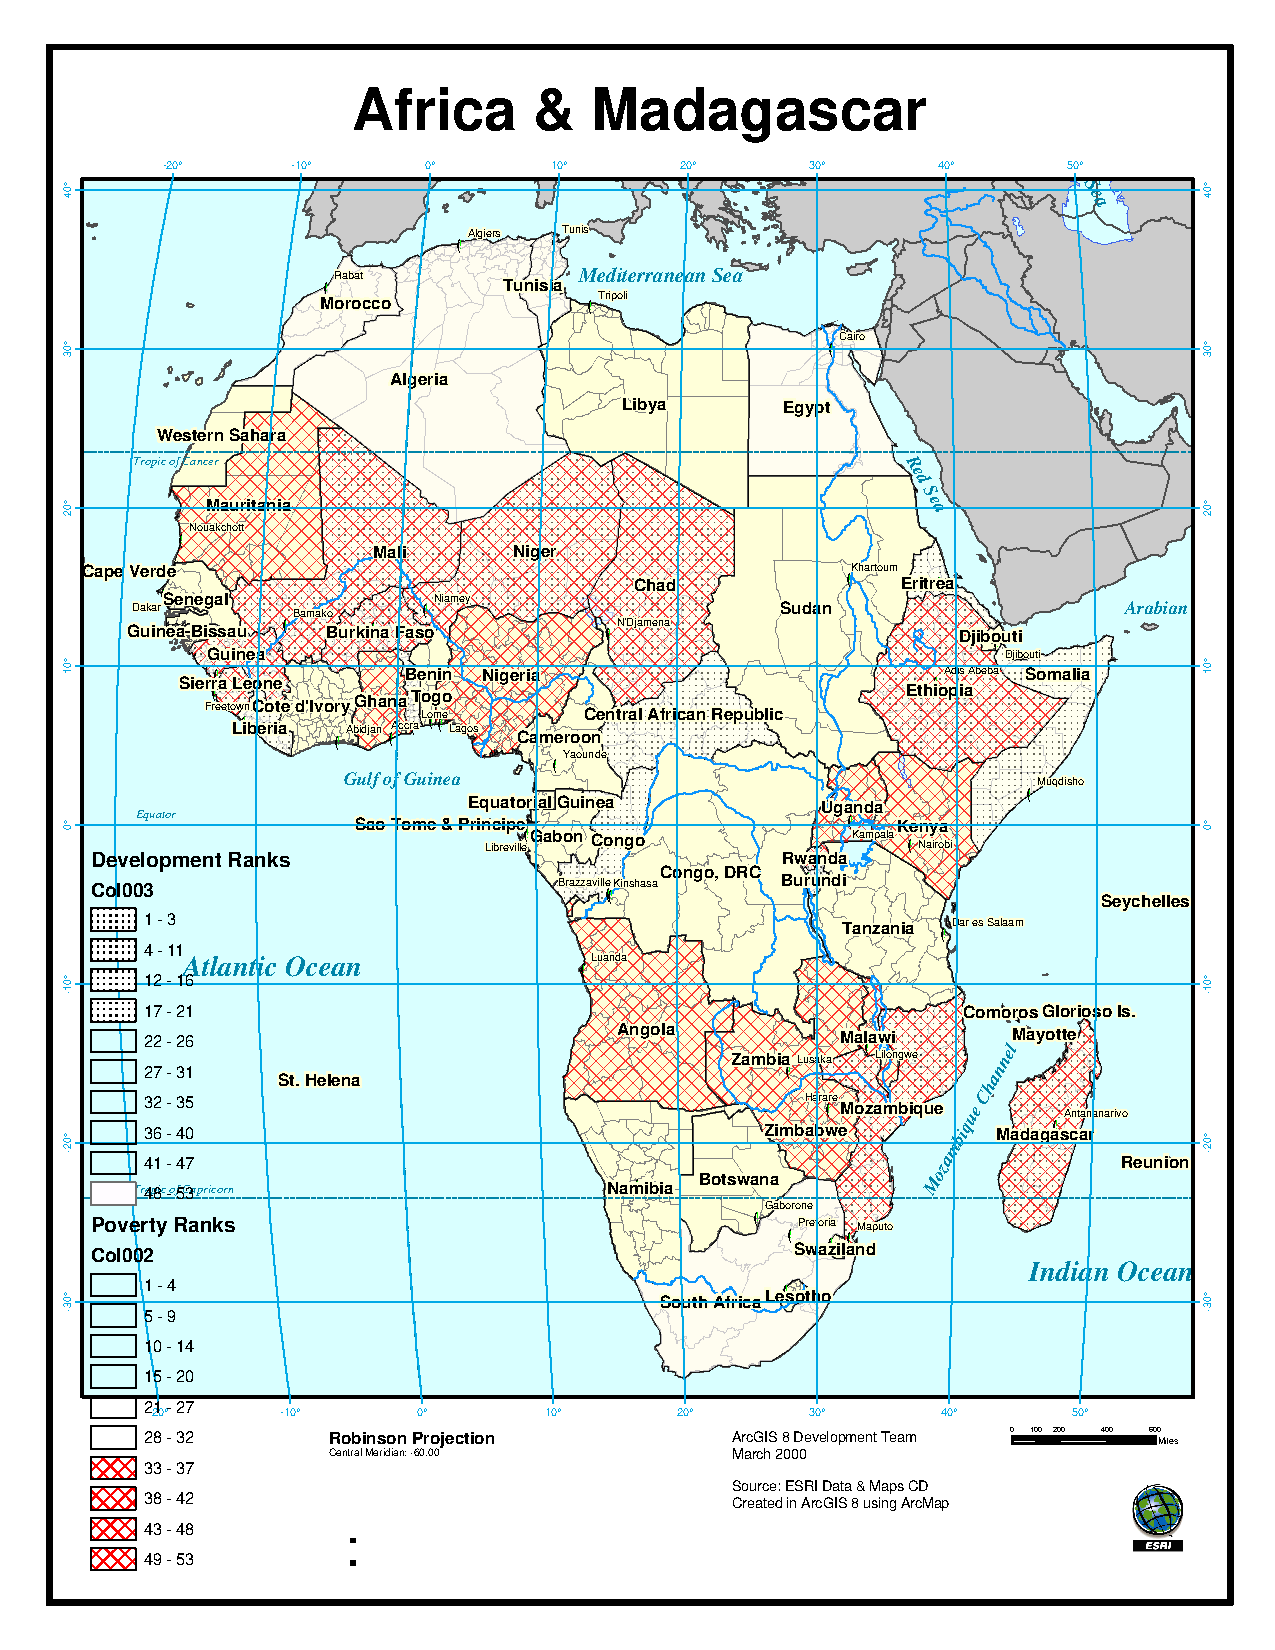
\includegraphics[width=6in]{Images/GIS/PovertyFeatureMapV2DevelopmentPovertyFloodFill.pdf}

\newpage

Poverty and Development ranks with State Population

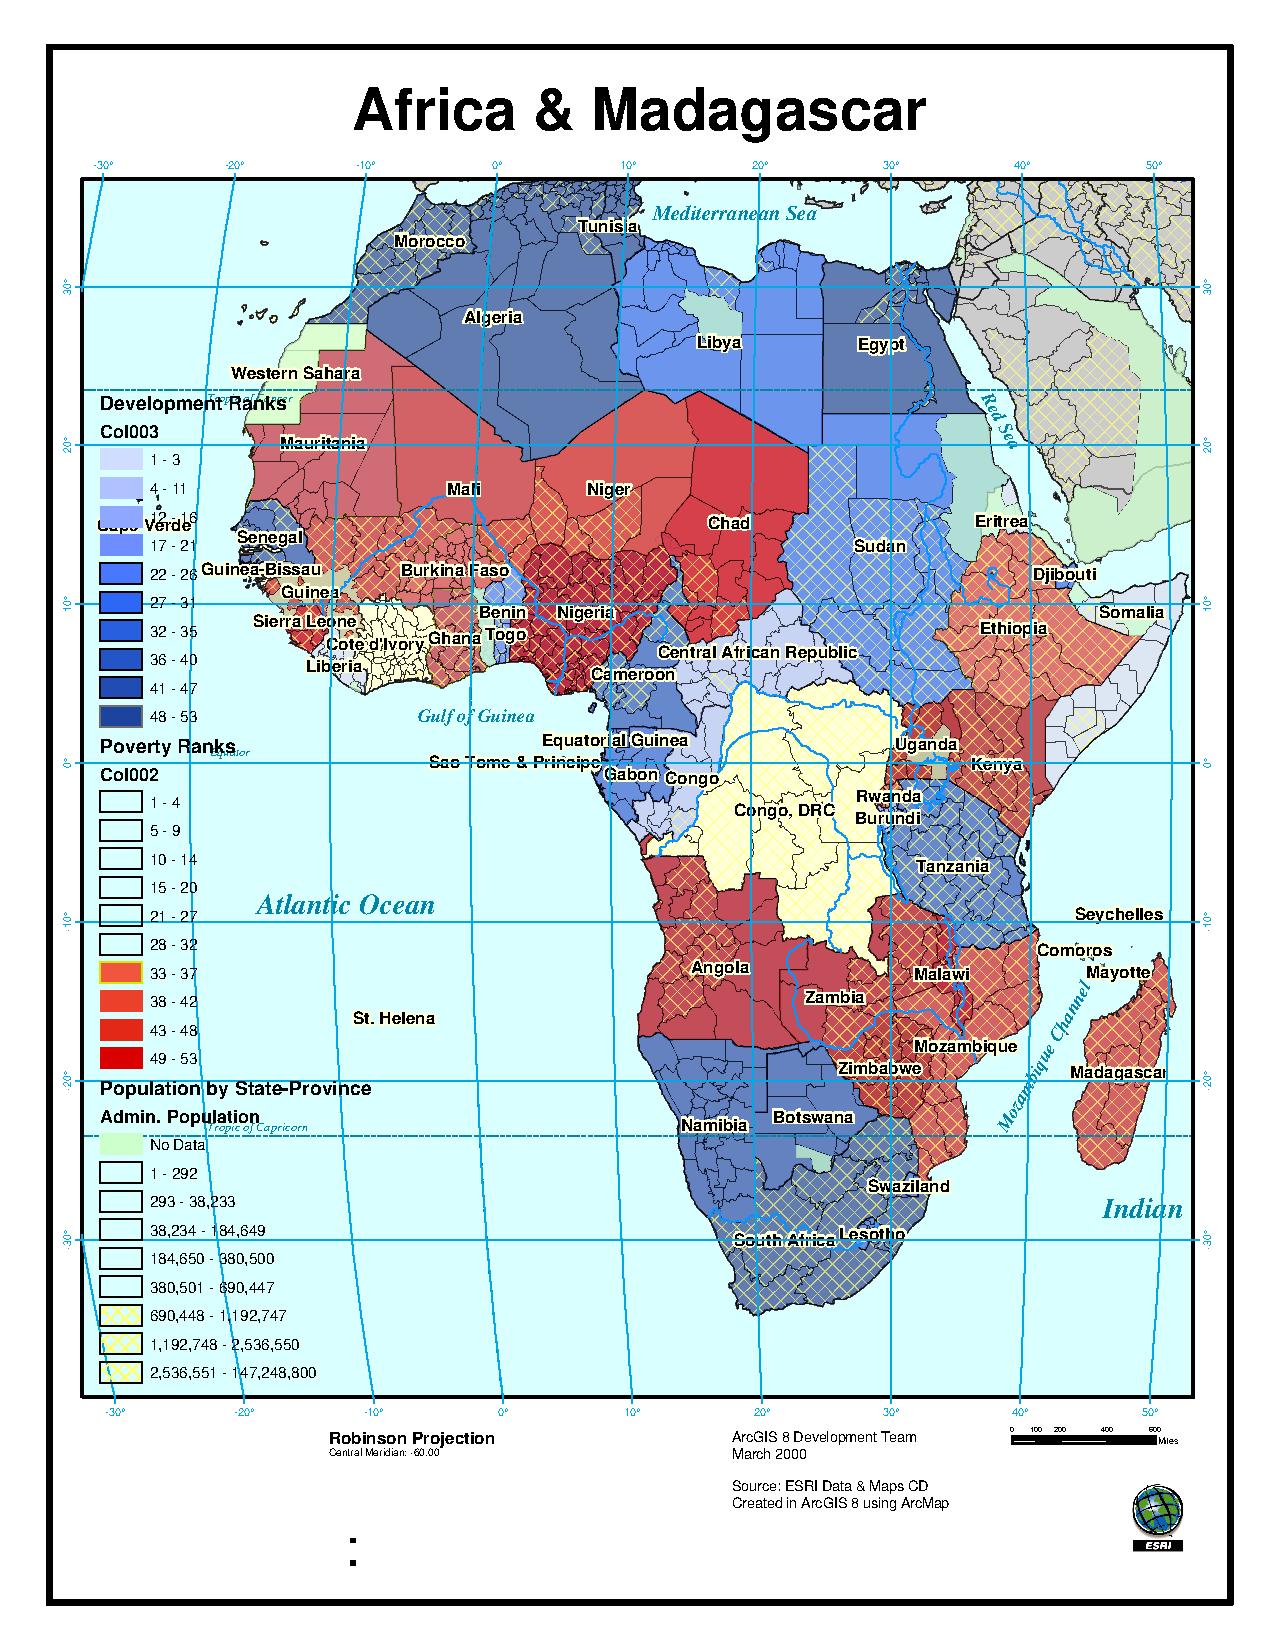
\includegraphics[width=5in]{Images/GIS/PovertyFeatureMapV4_PovertyDevelopment_StatePopulation.pdf}

\newpage

Another view of Poverty and Development ranks with State
Population

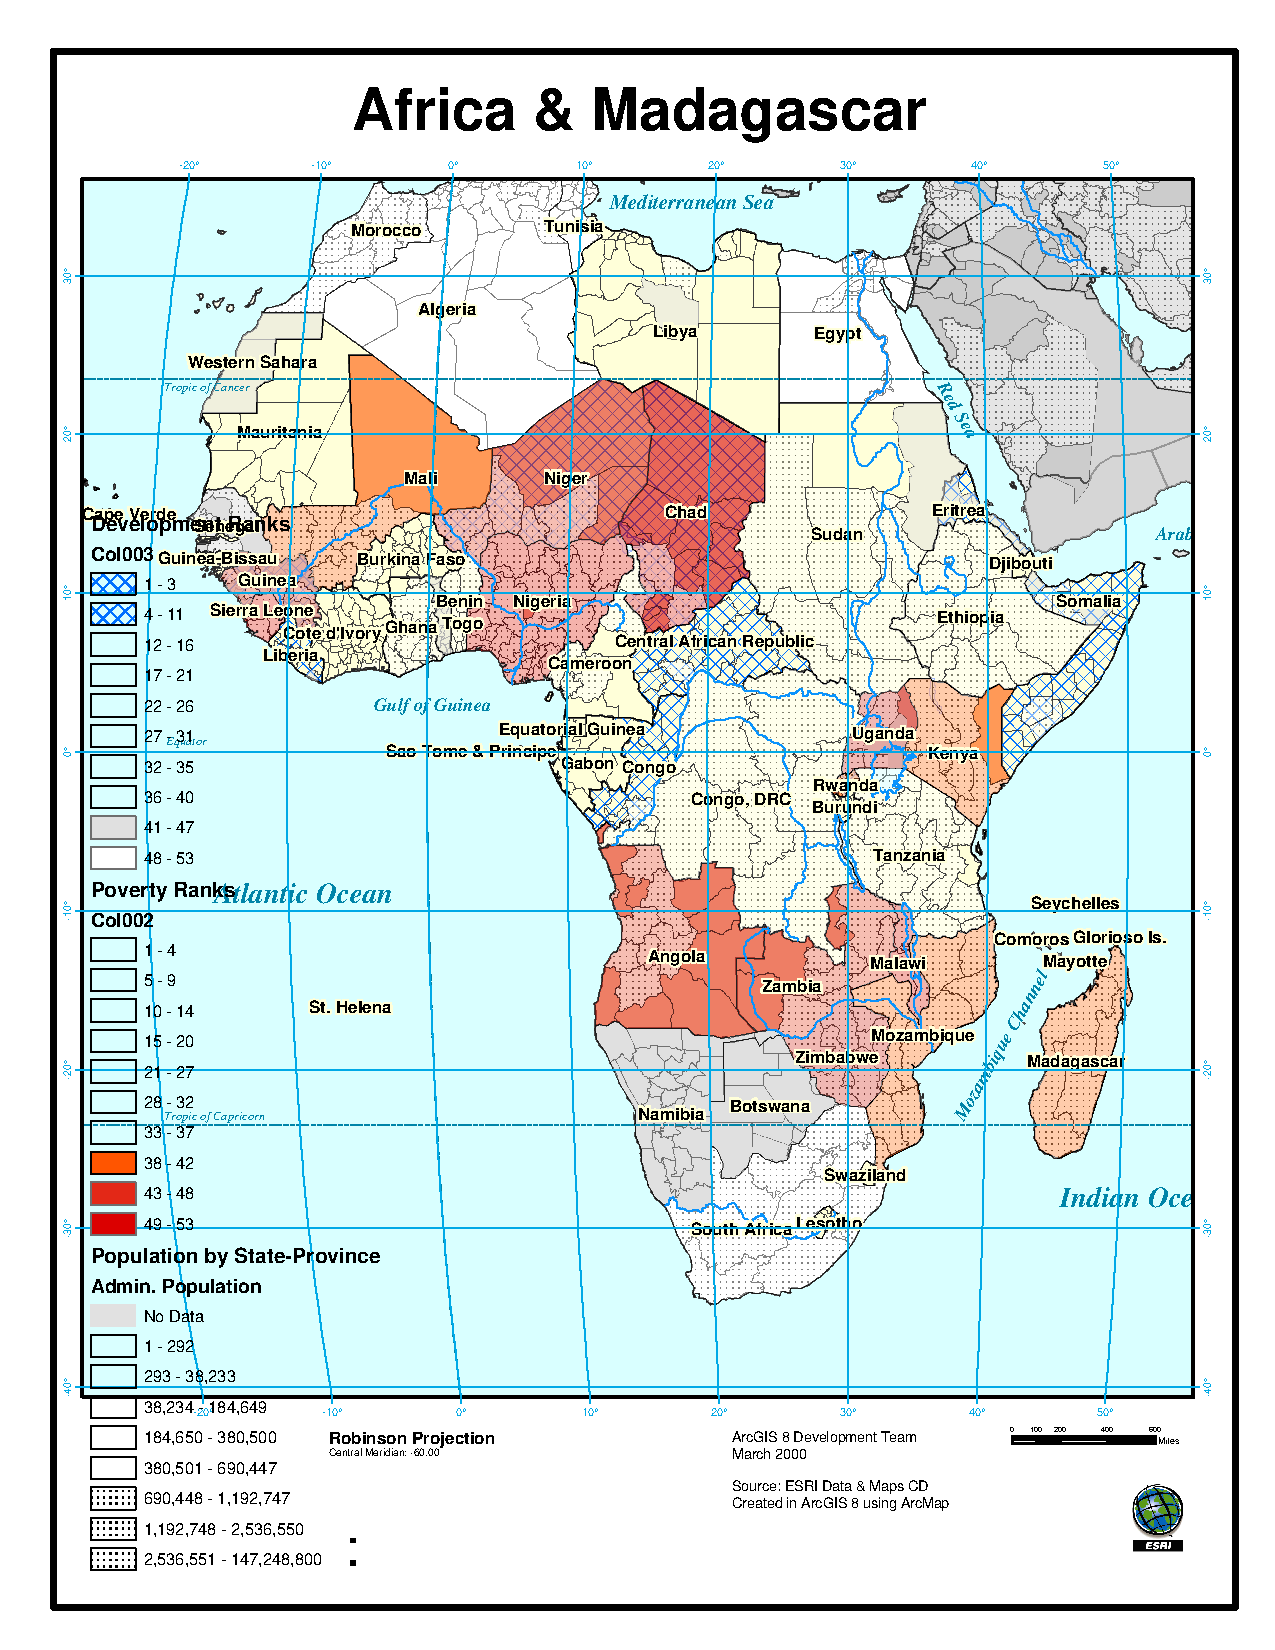
\includegraphics[width=5in]{Images/GIS/PovertyFeatureMapV9_PovertyDev_StatePop.pdf}

\newpage

Poverty, Habitat, and State Population (2000) - $>$ 200\% zoom
recommended.

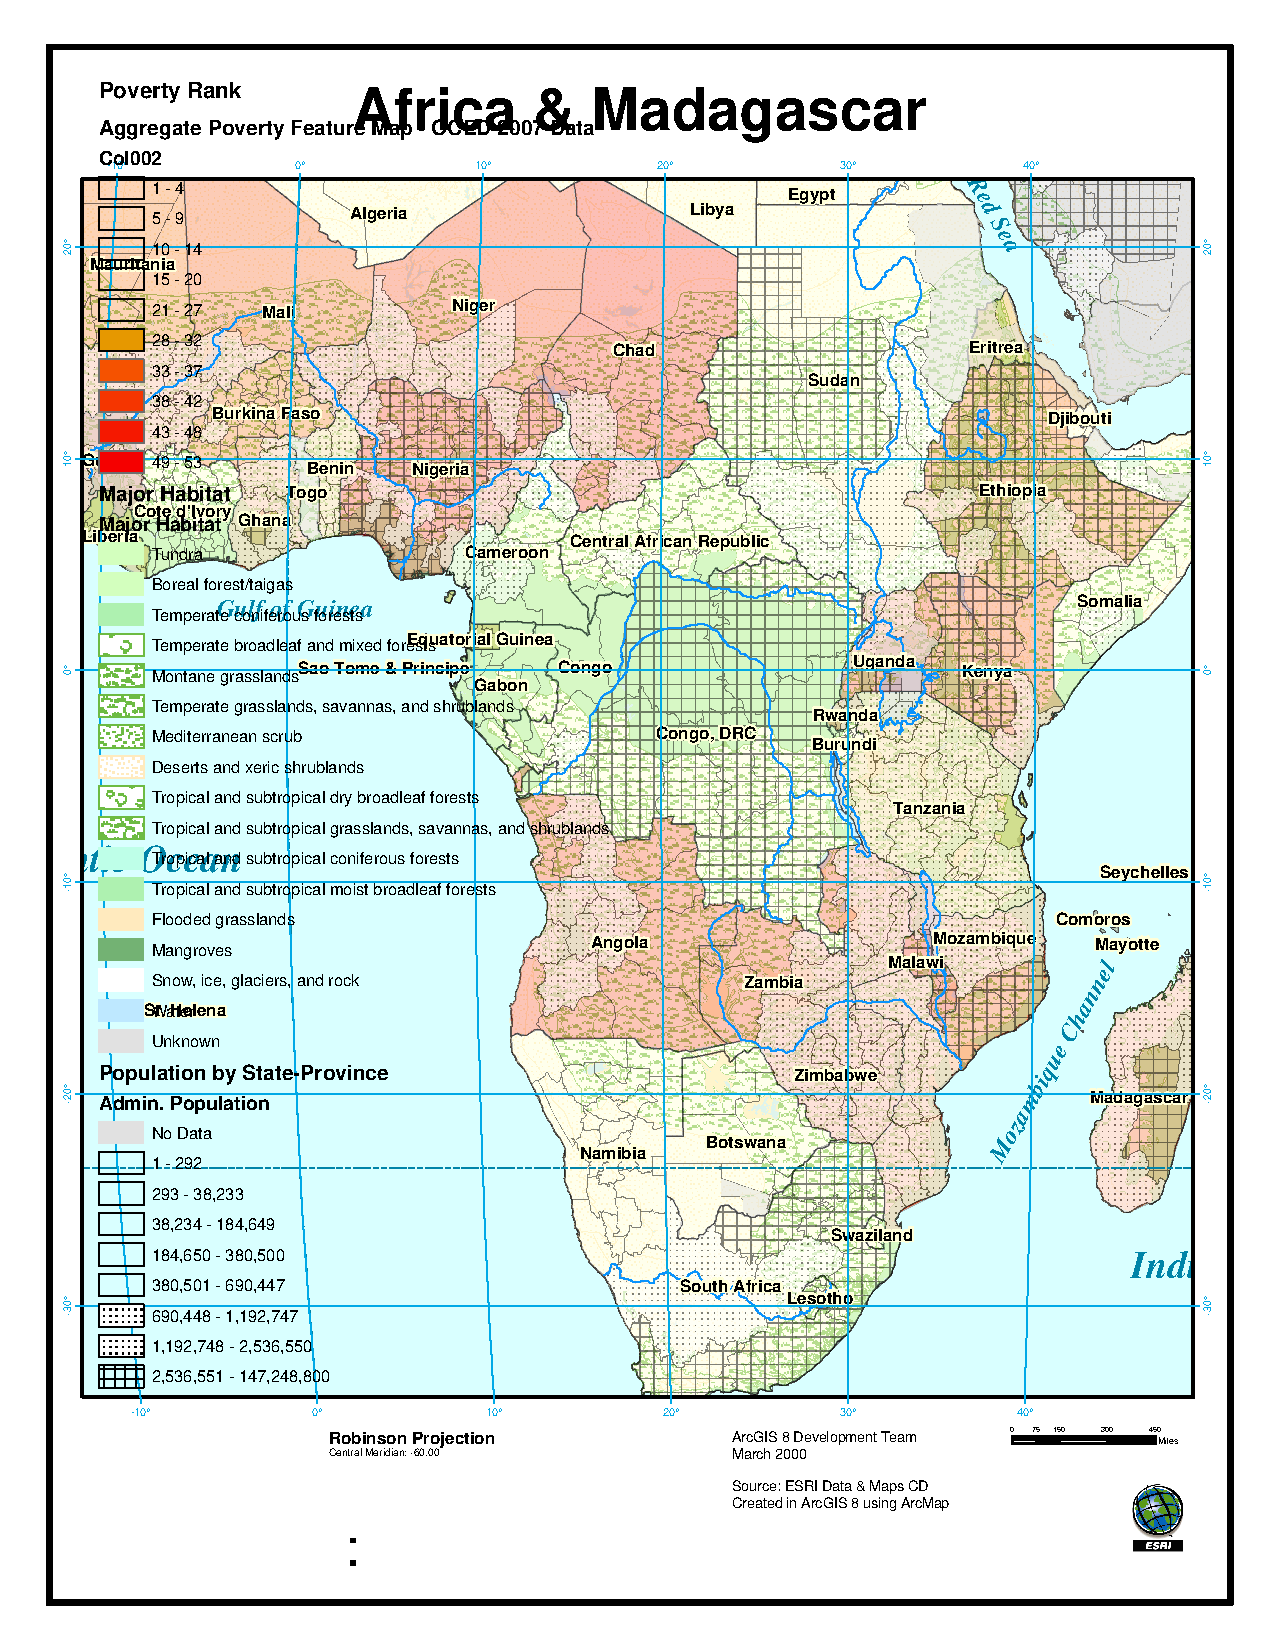
\includegraphics[width=5in]{Images/GIS/PovertyFeatureMapV5_Poverty_Habitat_StatePopulation.pdf}

\newpage

Older ESRI data showing similar spatial pattern using infant
mortality and exports.

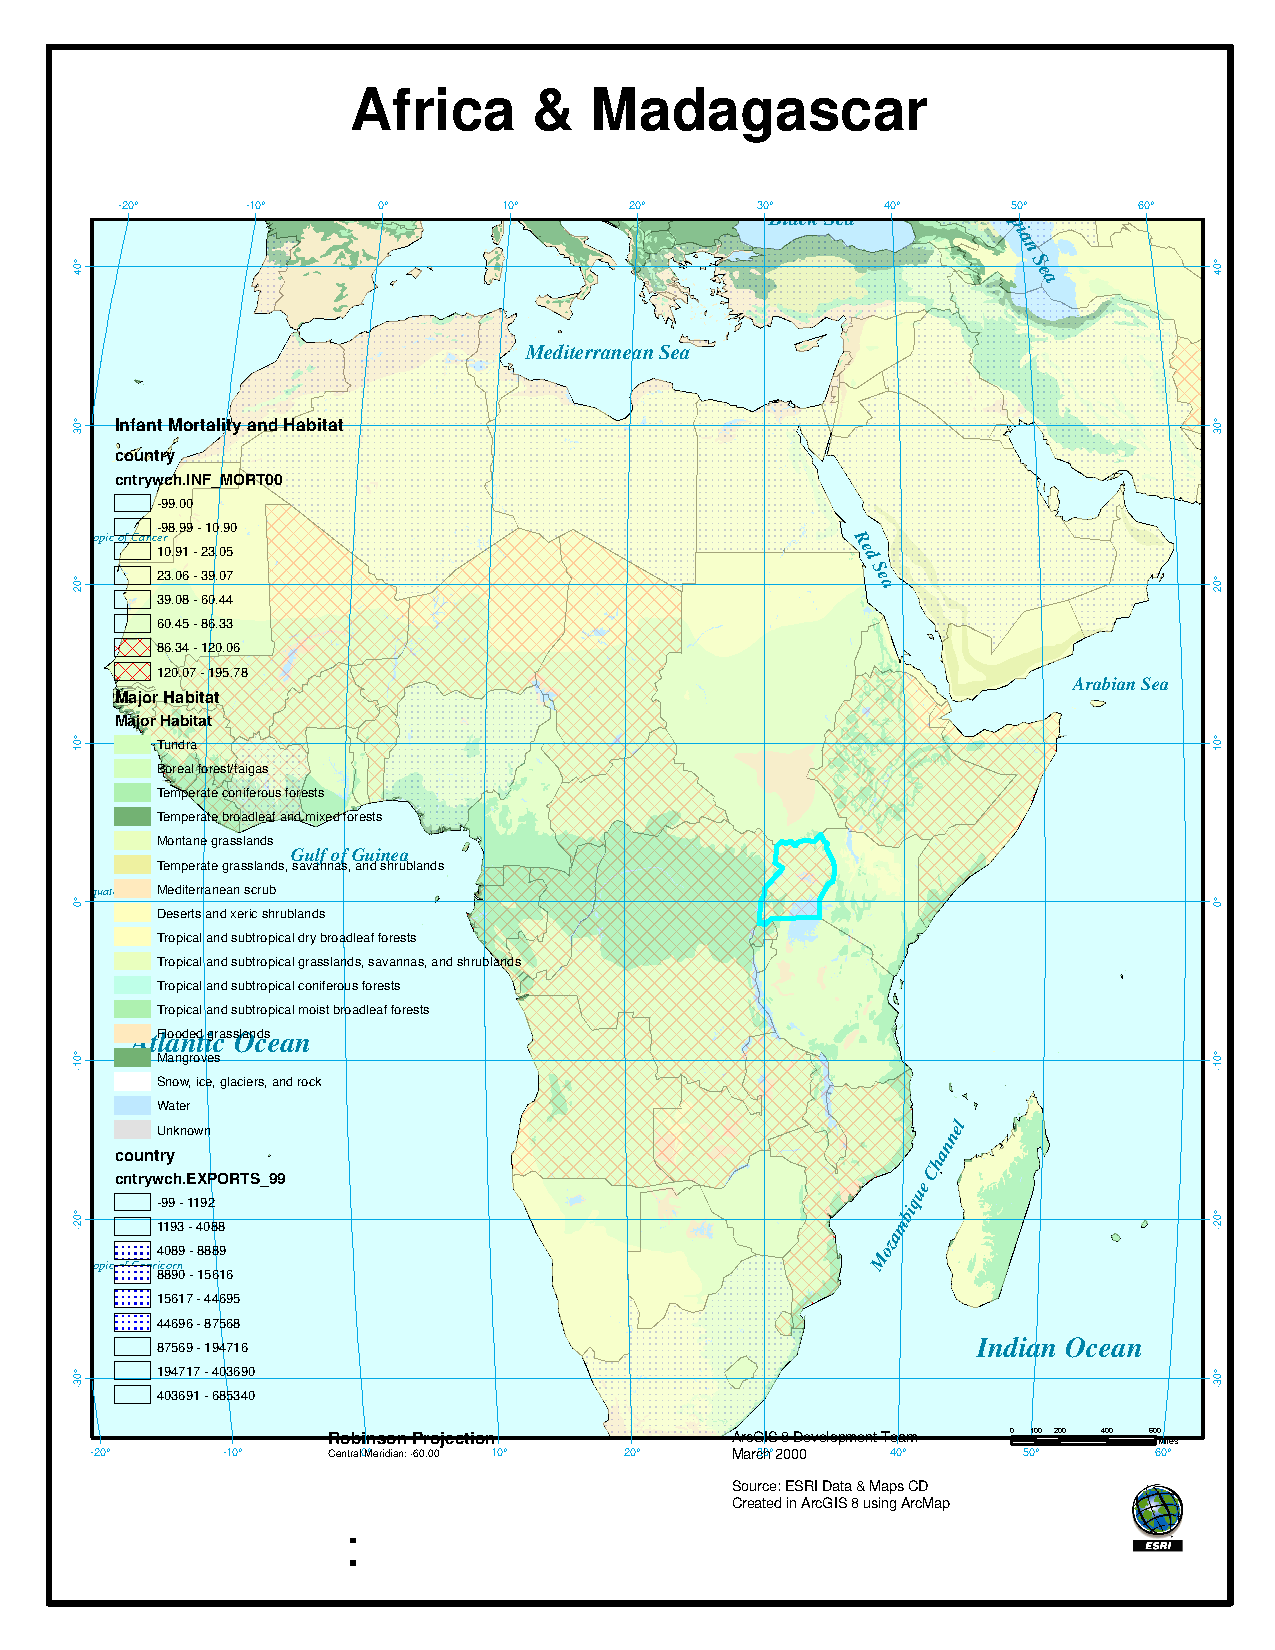
\includegraphics[width=5in]{Images/GIS/InfantMortality_X_Habitat_X_Exports_V9.pdf}

\newpage





%
%
%The Moran scatter plot provides a visual exploration of spatial
%autocorrelation (Anselin 1995, 1996, 2002). It is produced when
%you perform a univariate or bivariate local Moran analysis.
%Anselin (2002) describes this as "the spatial lag of the variable
%on the vertical axis and the original variable on the horizontal
%axis" (spatial lag being the values of its neighbors).
%
%You can obtain two different kinds of Moran scatter plots:
%
%Univariate (the same variable is plotted for the objects and their
%neighbors).
%
%Bivariate (one variable is plotted for the objects while another
%is plotted for neighbors).
%
%The Moran scatter plot displays standardized variables, not the
%raw data. Standardization is denoted by a (Z) after the variable
%name for z-score. While the strength of Moran�s I lies in its
%simplicity, its major limitations is that it tends to average
%local variations in the strength of spatial autocorrelation. This
%has prompted statisticians to develop local indices of spatial
%association. This category of tools examines the local level of
%spatial autocorrelation in order to identify areas where values of
%the variable are both extreme and geographically homogeneous. This
%approach is most useful when, in addition to global trends in the
%entire sample of observations, there exist also pockets of
%localities exhibiting homogeneous values that do not follow the
%global trend. This leads to identification of so-called hot spots
%-regions where the considered phenomenon is extremely pronounced
%across localities- as well of spatial outliers. The index fast
%becoming the standard tool to examine local autocorrelation is Luc
%Anselin�s LISA (local indicator of spatial association), which can
%be seen as the local equivalent of Moran�s I. the sum of all local
%indices is proportional to the (global) value of Moran�s
%statistic. The local value of a LISA is computed as:

%For each location, LISA values allow for the computation of
%its similarity with its neighbours and also to test its
%significance. Five scenarios may emerge: .. Locations with high
%values with similar neighbours: high-high. Also known as � hot
%spots �. .. Locations with low values with similar neighbours:
%low-low. Also known as � cold spots �. .. Locations with high
%values with low-value neighbours: high-low. Potential �spatial
%outliers�. .. Locations with low values with high-value
%neighbours: low-high. Potential �spatial outliers�. .. Locations
%with no significant local autocorrelation. These specific
%configurations can be first identified from a scatterplot showing
%observed values against the averaged value of their neighbours.
%This so-called Moran scatterplot is a useful exploratory tool.
%Once a significance level is set, values can also be plotted on a
%map to display the specific locations of hot spots and potential
%outliers.
%The four quadrants represent the four types of spatial association
%that exist: Quadrant I - high values of y surrounded by similarly
%high values; Quadrant II - low values of y surrounded by
%dissimilarly high values; Quadrant III � low values of y
%surrounded by similarly low values; Quadrant IV � high values of y
%surrounded by dissimilarly low values.
%Influential observations
%can be identified for their contributions, or leverage, by means
%of the two-sigma rule, or those observations falling more than two
%standard deviations from the origin



%The Moran scatter plot provides a visual exploration of spatial
%autocorrelation (Anselin 1995, 1996, 2002). It is produced when
%you perform a univariate or bivariate local Moran analysis.
%Anselin (2002) describes this as "the spatial lag of the variable
%on the vertical axis and the original variable on the horizontal
%axis" (spatial lag being the values of its neighbors).
%
%The four quadrants represent the four types of spatial association
%that exist: Quadrant I - high values of y surrounded by similarly
%high values; Quadrant II - low values of y surrounded by
%dissimilarly high values; Quadrant III � low values of y
%surrounded by similarly low values; Quadrant IV � high values of y
%surrounded by dissimilarly low values.

The following plots were generated in Matlab using Arc Mat ESRI
reader and The Spatial Econometrics Toolbox \footn{Arc Mat, a
Matlab toolbox for using ArcView Shape files for spatial
econometrics and statistics James P. LeSage, R. Kelley Pace}.  The
Moran Scatter plot provides a visual representation of spatial
autocorrelation. The corresponding map shows the groupings.  The
plot relates the variable to the spatial z-score.
\\\\

\begin{center}

 Linear Association \newline

 \begin{tabular}{|c|c|}
  \hline
  % after \\: \hline or \cline{col1-col2} \cline{col3-col4} ...
  - + (Green) &  + + (Red)\\
  \hline
  - - (Cyan) &  + - (Blue) \\
  \hline
\end{tabular}
\end{center}

\newpage

Moran autocorrelation maps for poverty rank data.  Red here is
poor near poor.

\begin{tabular}{ c}
\hline
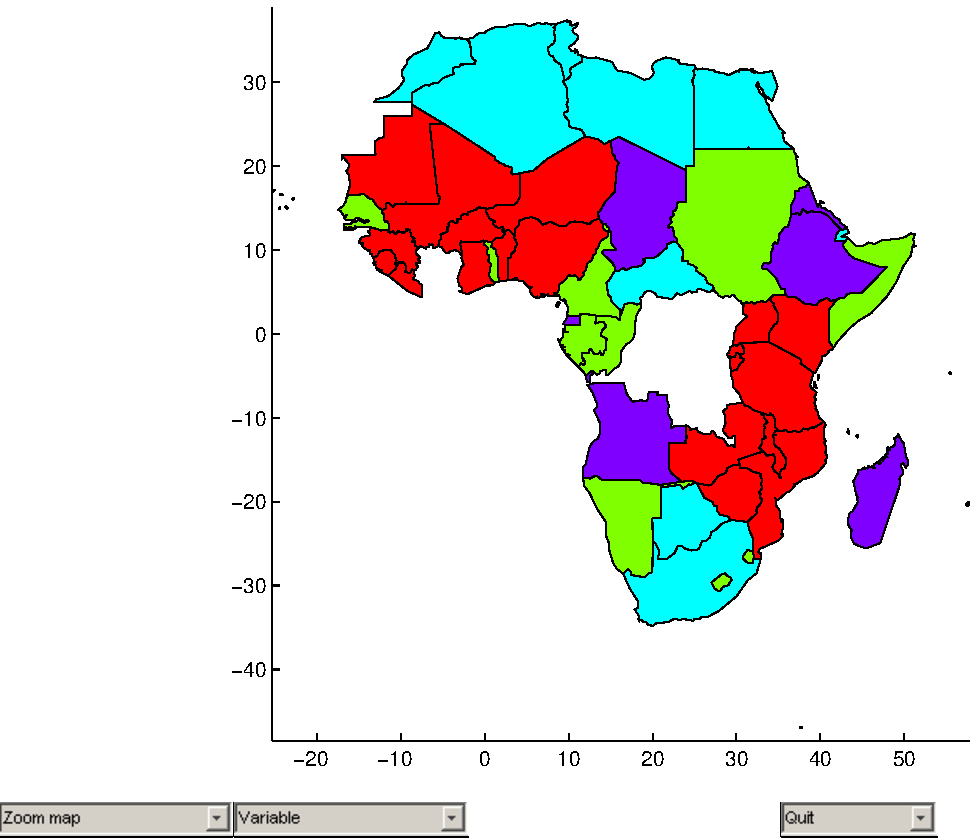
\includegraphics[width=4in]{Images/GIS/MoranMapForPovertyAggregateRanks.pdf}\\
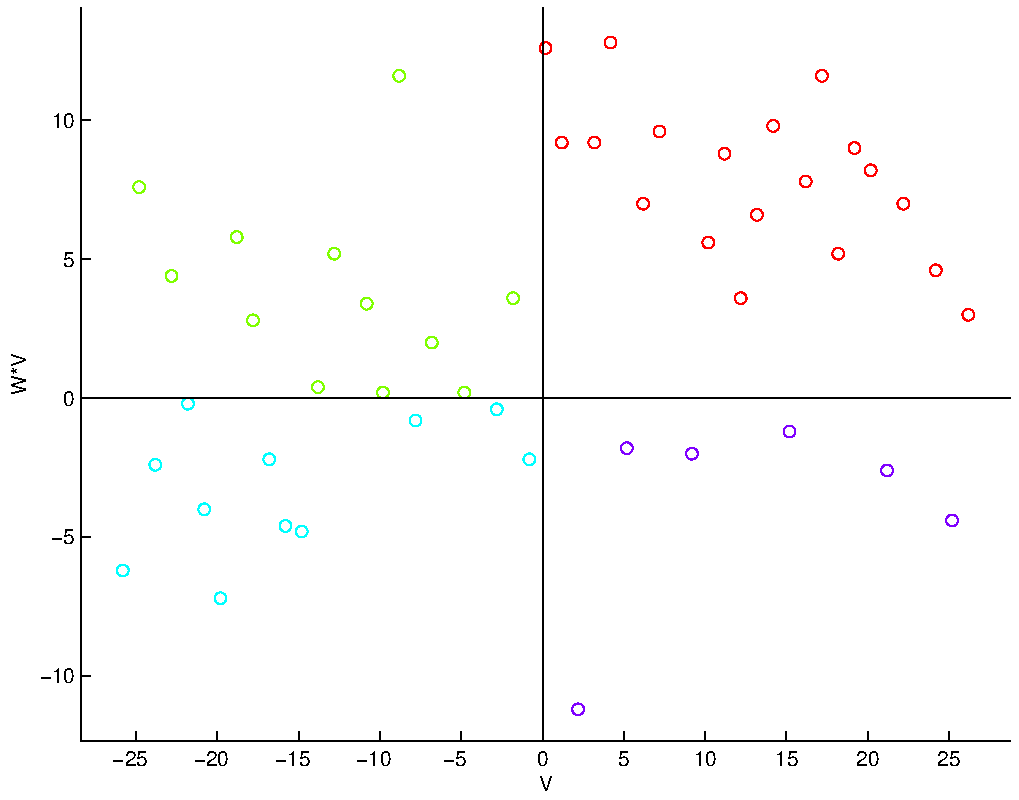
\includegraphics[width=4in]{Images/GIS/MoranScatterPlotForPovertyAggregateRanks.pdf}
\end{tabular}
\newpage

Moran autocorrelation maps for development rank data.  Red here is
a development hot spot.

\begin{tabular}{ c}
  % after \\: \hline or \cline{col1-col2} \cline{col3-col4} ...
   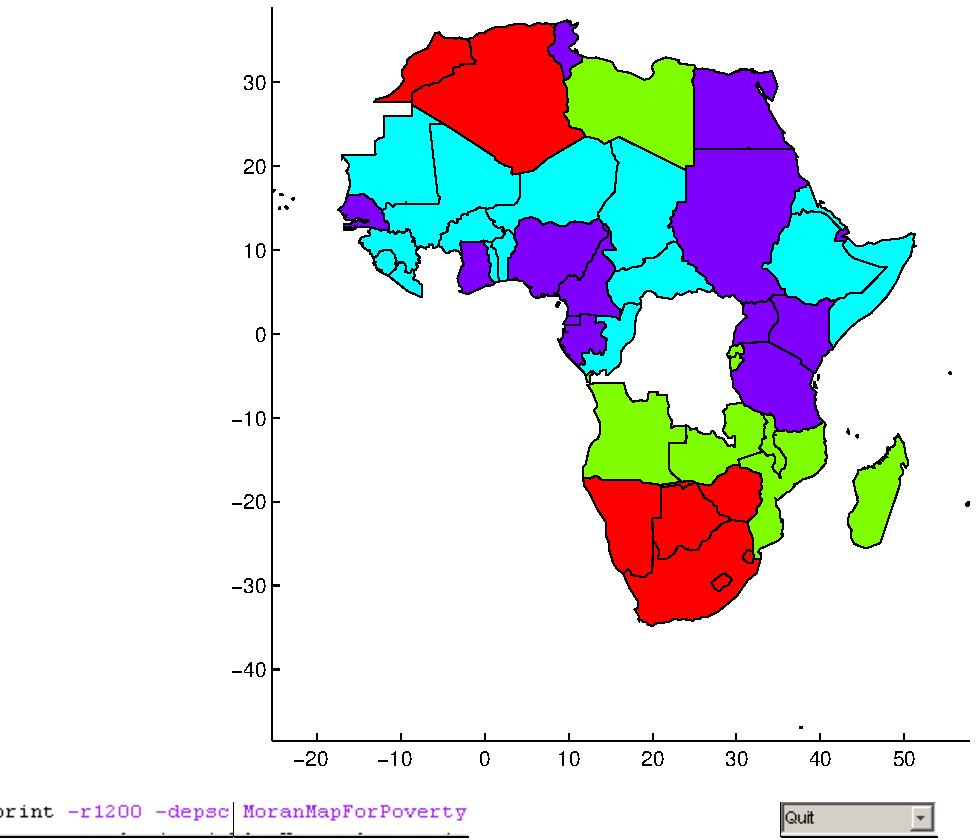
\includegraphics[width=4in]{Images/GIS/MoranMapForDevelopmentAggregateRanks.pdf}\\
  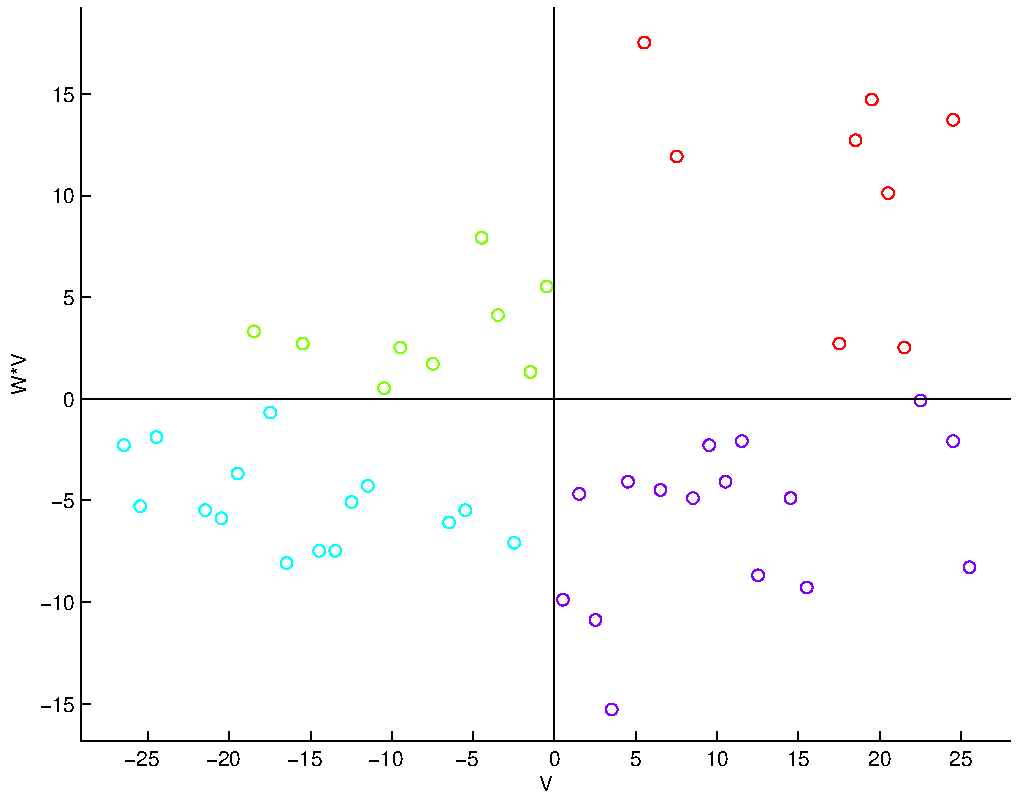
\includegraphics[width=4in]{Images/GIS/MoranScatterPlotForDevelopmentAggregateRanks.pdf}
\end{tabular}
